\section{Preprocessing}
\label{sec:preprocess}
\begin{figure}[!htb]
    \centering
    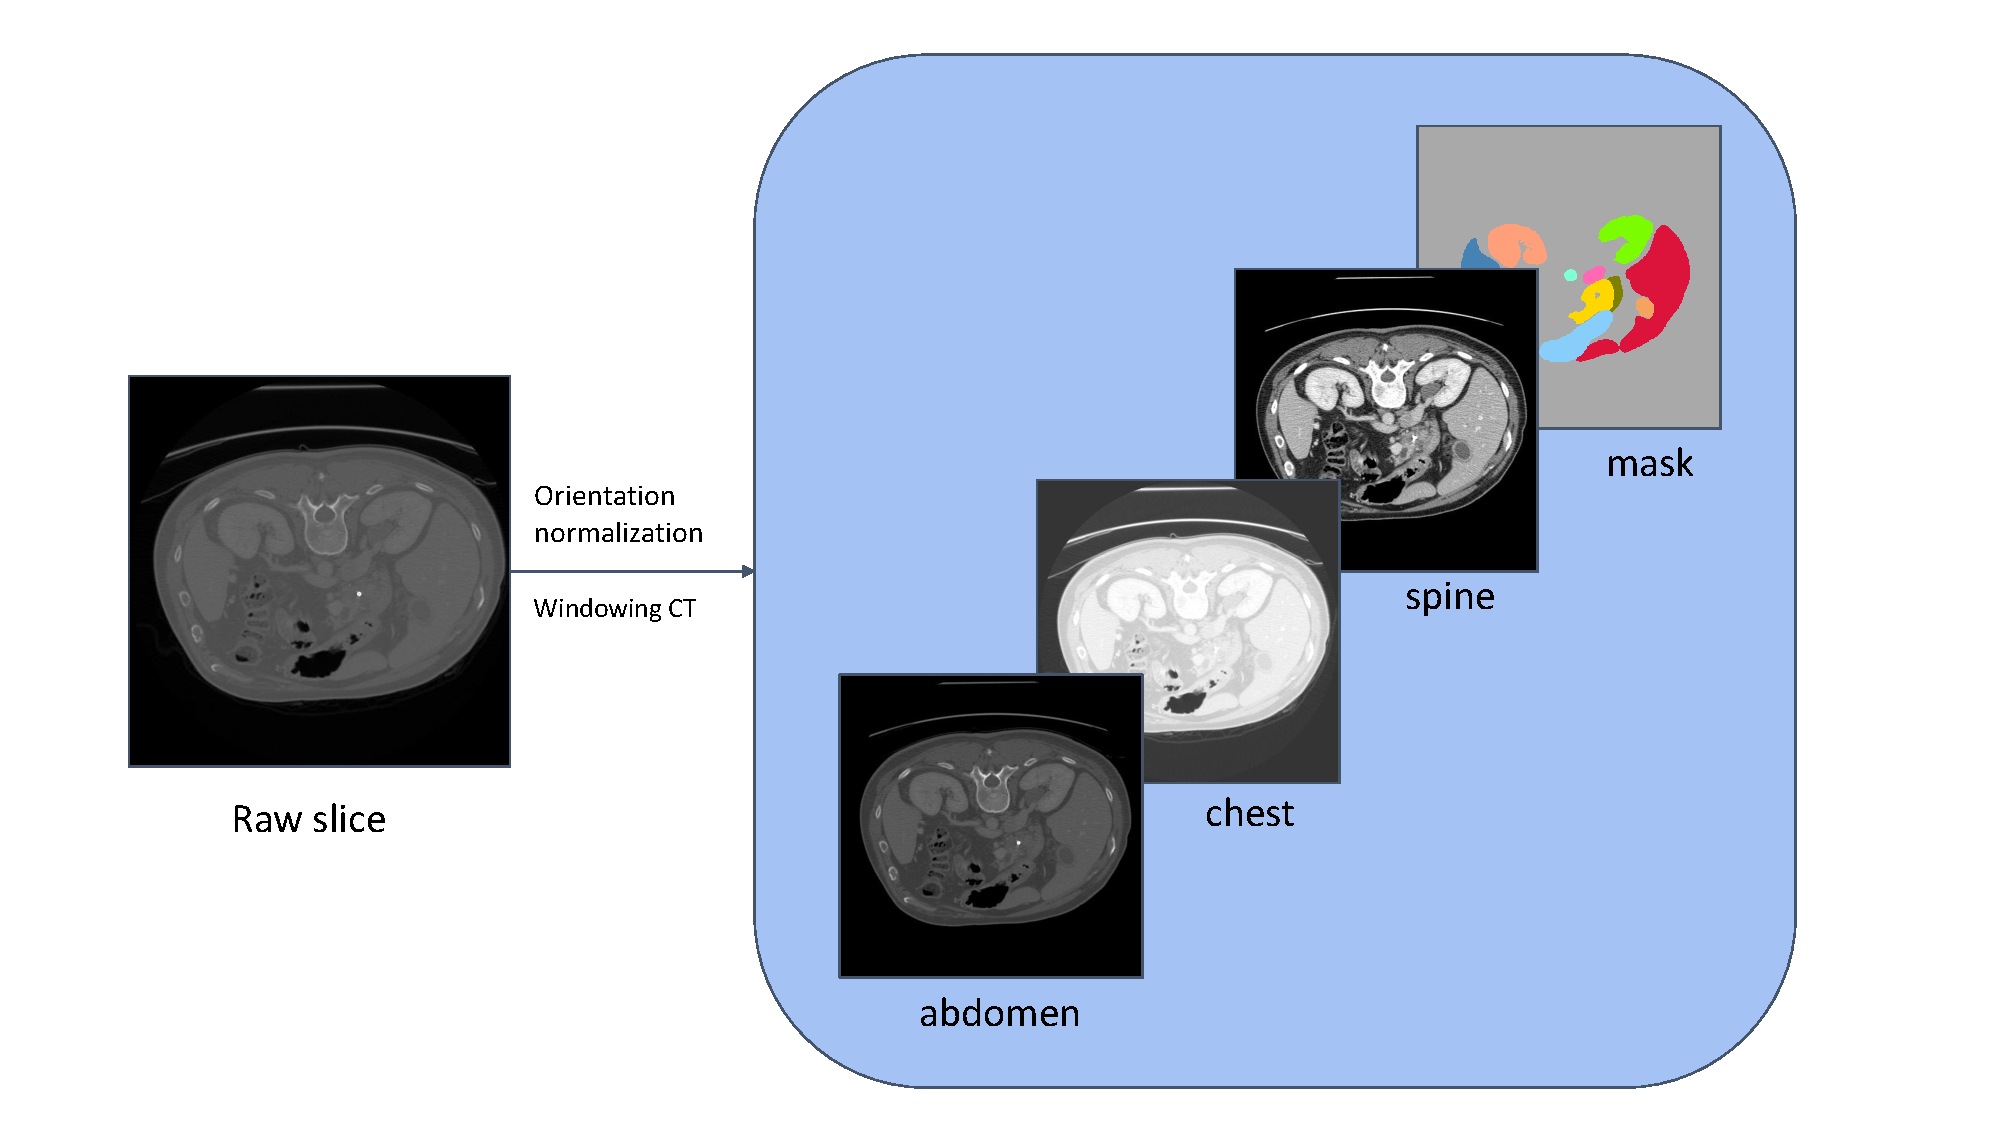
\includegraphics[width=\textwidth]{resources/new_images/preproc.pdf}
    \caption{Windowing CT.}
    \label{fig:windowingct}
\end{figure}

For preprocessing, we apply Windowing technique  \cite{windowingct17yahya} with different levels and widths to target specific parts of human organs. Windowing, also known as grey-level mapping, contrast stretching, histogram modification or contrast enhancement is the process in which the CT image grayscale component of an image is manipulated via the CT numbers; doing this will change the appearance of the picture to highlight particular structures. The brightness of the image is adjusted via the window level. The contrast is adjusted via the window width. In or experiments, we create 3 different versions of a single slice by highlight the abdomen, chest, and spine groups and stack it to one as a three-channel image (Fig. \ref{fig:preproc}). 

In addition, we choose the axial plane to cut the slices from the CT volumes since this plane has various dimension sizes. 
Due to some relatively small organs, it might be better to keep the original size of the slices without any cropping, resampling, or resizing methods.
The image is rotated to a predefined angle, then divided by 255 for normalization before going through the next step.